\begin{flushright} {\tiny {\color{gray} quadrature.tex}} \end{flushright}
%~~~~~~~~~~~~~~~~~~~~~~~~~~~~~~~~~~~~~~~~~~~~~~~~~~~~~~~~~~~~~~~~~~~~~~~~~~~~~~~~~~~~~~~~~~~~~~~~~~

As we will see later, using the Finite Element method to solve problems involves 
computing integrals which are more often than not too complex to be computed 
analytically/exactly. We will then need to compute them numerically.

[wiki] In essence, 
the basic problem in numerical integration is to compute an approximate solution to a definite integral
\begin{equation}
I=\int_a^b f(x) dx
\label{Idef}
\end{equation}
to a given degree of accuracy.
This problem has been widely studied and we know that 
if $f(x)$ is a smooth function, and the domain of integration is bounded, 
there are many methods for approximating the integral to the desired precision.

There are several reasons for carrying out numerical integration.
\begin{itemize}
\item The integrand $f(x)$ may be known only at certain points, such as obtained by sampling. 
Some embedded systems and other computer applications may need numerical integration for this reason.
\item A formula for the integrand may be known, but it may be difficult or impossible to 
find an antiderivative that is an elementary function. An example of such an integrand 
is $f(x)=\exp(-x^2)$, the antiderivative of which (the error function, times a constant) 
cannot be written in elementary form.
\item It may be possible to find an antiderivative symbolically, but it may be 
easier to compute a numerical approximation than to compute the antiderivative. That may be the 
case if the antiderivative is given as an infinite series or product, or if its evaluation 
requires a special function that is not available.
\end{itemize}

Let us remember that the integral of Eq.~\eqref{Idef} is in fact equal to the (signed) area 
between the $x$-axis and the curve $f(x)$ over the interval $[a,b]$:

\begin{flushright} {\tiny {\color{gray} (tikz\_quadrature\_idef.tex)}} \end{flushright}
%~~~~~~~~~~~~~~~~~~~~~~~~~~~~~~~~~~~~~~~~~~~~~~~~~~~~~~~~~~~~~~~~~~~~~~~~~~~~~~~~~~~~~~~~~~~~~~~~~~

\begin{center}
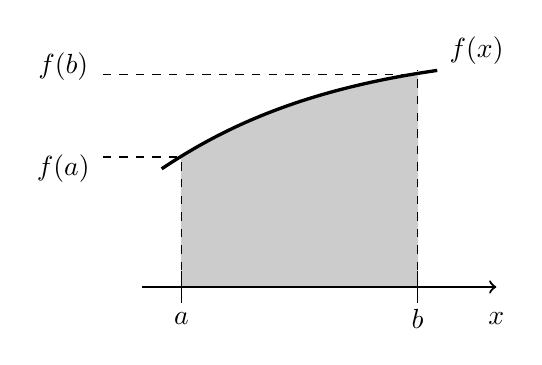
\begin{tikzpicture}
%\draw[step=0.5cm,gray,very thin] (0,0) grid (7,5); 
\draw[fill=gray!20,gray!40] (1,1)--(4,1)--(4,3.7)--(3.25,3.55)--(2.5,3.35)--(1.75,3.05)--(1,2.65)--cycle;
\draw [thick,->] (0.5,1) -- (5,1);
\node[] at (1,0.6) {$a$};
\node[] at (4,0.6) {$b$};
\node[] at (5,0.6) {$x$};
\draw [-] (1,0.8) -- (1,1.2);
\draw [-] (4,0.8) -- (4,1.2);
\draw [dashed] (1,1) -- (1,2.6);
\draw [dashed] (4,1) -- (4,3.75);
\draw[very thick] (0.75,2.5) .. controls (1.5,3) and (2.5,3.5) .. (4.25,3.75);
\node[] at (4.75,4) {$f(x)$};
\node[] at (-0.5,2.5) {$f(a)$};
\draw [dashed] (0,2.65) -- (1,2.65);
\node[] at (-0.5,3.8) {$f(b)$};
\draw [dashed] (0,3.7) -- (4,3.7);
\end{tikzpicture}
\end{center}



Note that in the example above $f(x)>0$ so the area of the gray domain is counted positive.
For example, if the function $f(x)$ is a polynomial the integral can easily be computed 
analytically. In the case of a $0^{th}$ order polynomial, we have $f(x)=C$ where $C$ is a 
constant. We then have 
\begin{equation}
I=\int_a^b f(x) dx = \int_a^b C \; dx  = C \int_a^b dx = C(b-a)
\end{equation}

\begin{flushright} {\tiny {\color{gray} (tikz\_quadrature\_idef2.tex)}} \end{flushright}
%~~~~~~~~~~~~~~~~~~~~~~~~~~~~~~~~~~~~~~~~~~~~~~~~~~~~~~~~~~~~~~~~~~~~~~~~~~~~~~~~~~~~~~~~~~~~~~~~~~


\begin{center}
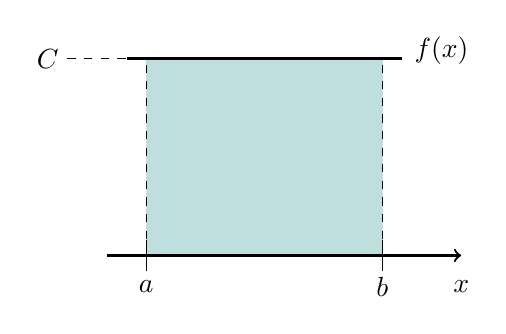
\begin{tikzpicture}
%\draw[step=0.5cm,gray,very thin] (0,0) grid (7,5); 
\draw[fill=teal!25,teal!25] (1,1)--(4,1)--(4,3.5)--(1,3.5)--cycle;
\draw [thick,->] (0.5,1) -- (5,1);
\node[] at (1,0.6) {$a$};
\node[] at (4,0.6) {$b$};
\node[] at (5,0.6) {$x$};
\draw [-] (1,0.8) -- (1,1.2);
\draw [-] (4,0.8) -- (4,1.2);
\draw [dashed] (1,1) -- (1,3.5);
\draw [dashed] (4,1) -- (4,3.5);
\draw[very thick] (0.75,3.5) --(4.25,3.5);
\node[] at (4.75,3.6) {$f(x)$};
\draw [dashed] (0,3.5) -- (4,3.5);
\node[] at (-0.25,3.5) {$C$};
\end{tikzpicture}
\end{center}






We see that the area of the gray domain in simply the product of its length $b-a$ by its height $c$
and we indeed recover $I=C(b-a)$.


%-------------------------------------------------------------------------
\subsubsection{in 1D - Midpoint and Trepezoidal rules  \label{sec:quad1D}}

The simplest method of this type is to let the interpolating function be 
a constant function (a polynomial of degree zero) that passes through the point $((a+b)/2, f((a+b)/2))$.
This is called the midpoint rule \index{general}{Midpoint Rule} or rectangle rule. 
\index{general}{Rectangle Rule}
We then have 
\[
I=\int_a^b f(x)dx \simeq (b-a) f\left(\frac{a+b}{2}\right)
\]
which is the area of this gray domain:

\begin{flushright} {\tiny {\color{gray} (tikz\_quadrature\_rectangle.tex)}} \end{flushright}
%~~~~~~~~~~~~~~~~~~~~~~~~~~~~~~~~~~~~~~~~~~~~~~~~~~~~~~~~~~~~~~~~~~~~~~~~~~~~~~~~~~~~~~~~~~~~~~~~~~

\begin{center}
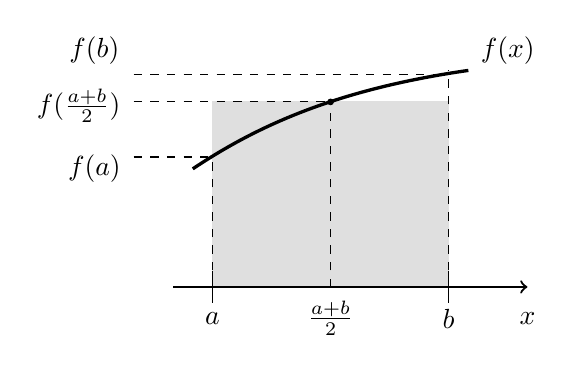
\begin{tikzpicture}
%\draw[step=0.5cm,gray,very thin] (0,0) grid (7,5); 
\draw[fill=gray!25,gray!25](1,1) rectangle (4,3.35);
\draw [thick, ->] (0.5,1) -- (5,1);
\node[] at (1,0.6) {$a$};
\node[] at (4,0.6) {$b$};
\node[] at (5,0.6) {$x$};
\node[] at (2.5,0.6) {$\frac{a+b}{2}$};
\draw [-] (1,0.8) -- (1,1.2);
\draw [-] (4,0.8) -- (4,1.2);
\draw [dashed] (1,1) -- (1,2.6);
\draw [dashed] (2.5,1) -- (2.5,3.35);
\draw [dashed] (4,1) -- (4,3.75);
\draw[black,fill=black] (2.5,3.35)   circle (1pt);
\draw[very thick] (0.75,2.5) .. controls (1.5,3) and (2.5,3.5) .. (4.25,3.75);
\node[] at (4.75,4) {$f(x)$};
\node[] at (-0.7,3.3) {$f(\frac{a+b}{2})$};
\draw [dashed] (0,3.35) -- (2.5,3.35);
\node[] at (-0.5,2.5) {$f(a)$};
\draw [dashed] (0,2.65) -- (1,2.65);
\node[] at (-0.5,4) {$f(b)$};
\draw [dashed] (0,3.7) -- (4,3.7);
\end{tikzpicture}
\end{center}



We can do a little bit better at virtually no cost:
we choose the interpolating function to be a straight line 
(an affine function, i.e. a polynomial of degree 1)
passing through the points $(a, f(a))$ and $(b, f(b))$.
This is called the trapezoidal rule. \index{general}{Trapezoidal Rule} 
Then 
\[
I=\int_a^b f(x)dx \simeq (b-a) \frac{f(a)+f(b)}{2}
\]

\begin{flushright} {\tiny {\color{gray} (tikz\_quadrature\_trapeze.tex)}} \end{flushright}
%~~~~~~~~~~~~~~~~~~~~~~~~~~~~~~~~~~~~~~~~~~~~~~~~~~~~~~~~~~~~~~~~~~~~~~~~~~~~~~~~~~~~~~~~~~~~~~~~~~



\begin{center}
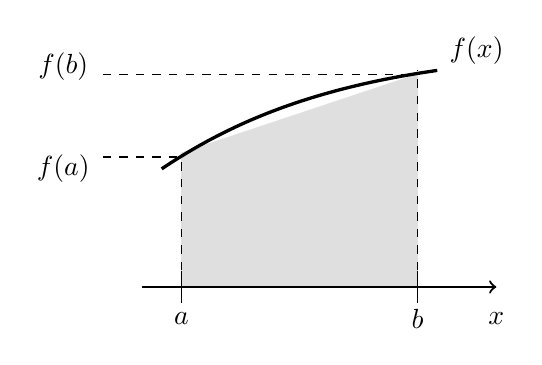
\begin{tikzpicture}
%\draw[step=0.5cm,gray,very thin] (0,0) grid (7,5); 
\draw[fill=gray!25,gray!25] (1,1)--(4,1)--(4,3.7)--(1,2.7)--cycle;
\draw [thick, ->] (0.5,1) -- (5,1);
\node[] at (1,0.6) {$a$};
\node[] at (4,0.6) {$b$};
\node[] at (5,0.6) {$x$};
\draw [-] (1,0.8) -- (1,1.2);
\draw [-] (4,0.8) -- (4,1.2);
\draw [dashed] (1,1) -- (1,2.6);
\draw [dashed] (4,1) -- (4,3.75);
\draw[very thick] (0.75,2.5) .. controls (1.5,3) and (2.5,3.5) .. (4.25,3.75);
\node[] at (4.75,4) {$f(x)$};
\node[] at (-0.5,2.5) {$f(a)$};
\draw [dashed] (0,2.65) -- (1,2.65);
\node[] at (-0.5,3.8) {$f(b)$};
\draw [dashed] (0,3.7) -- (4,3.7);
\end{tikzpicture}
\end{center}



We see that if the function $f$ is monotonous on the interval $[a,b]$ then 
the trapezoidal approach is likely to return a value close to the real value. 
However if the function $f$ oscillates a lot in the interval, approximating it 
with a single rectangle or trapeze is not a sound assumption.
We can then make use of the additive property of the integral: let $c$ 
be the coordinate of the middle of the $[a,b]$ interval, i.e. $c=(a+b)/2$. 
Then we have 
\[
I=\int_a^b f(x)dx = \int_a^c f(x)dx + \int_c^b f(x)dx
\]
We can then apply the midpoint rule or the trapezoidal rule over both segments 
$[a,c]$ and $[c,b]$:

\begin{flushright} {\tiny {\color{gray} (tikz\_quadrature\_both.tex)}} \end{flushright}
%~~~~~~~~~~~~~~~~~~~~~~~~~~~~~~~~~~~~~~~~~~~~~~~~~~~~~~~~~~~~~~~~~~~~~~~~~~~~~~~~~~~~~~~~~~~~~~~~~~

\begin{center}
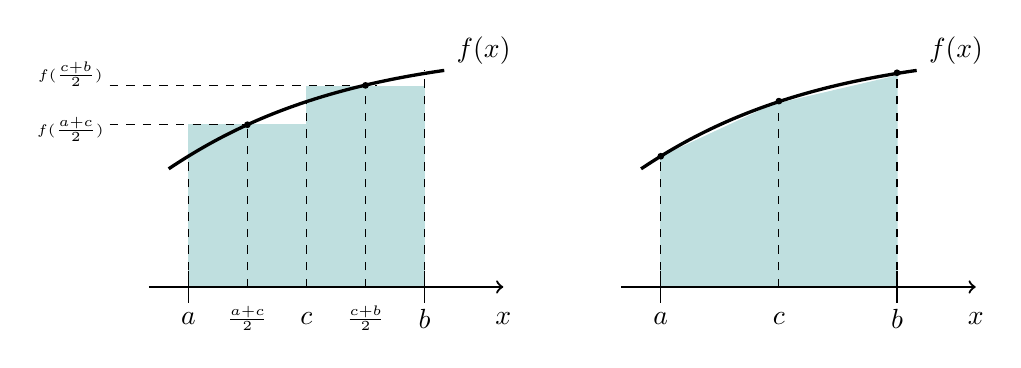
\begin{tikzpicture}
%\draw[step=0.5cm,gray,very thin] (0,0) grid (12,5); 
\draw[fill=teal!25,teal!25](1,1) rectangle (2.5,3.06);
\draw[fill=teal!25,teal!25](2.5,1) rectangle (4,3.55);
\draw [thick, ->] (0.5,1) -- (5,1);
\node[] at (1,0.6) {$a$};
\node[] at (4,0.6) {$b$};
\node[] at (5,0.6) {$x$};
\node[] at (2.5,0.6) {$c$};
\node[] at (1.75,0.6) {\tiny $\frac{a+c}{2}$};
\node[] at (3.25,0.6) {\tiny $\frac{c+b}{2}$};
\draw [-] (1,0.8) -- (1,1.2);
\draw [-] (4,0.8) -- (4,1.2);
\draw [dashed] (1,1) -- (1,2.6);
\draw [dashed] (2.5,1) -- (2.5,3.35);
\draw [dashed] (4,1) -- (4,3.75);
\draw [dashed] (1.75,1) -- (1.75,3.06);
\draw [dashed] (3.25,1) -- (3.25,3.56);
\draw[black,fill=black] (1.75,3.06)  circle (1pt);
\draw[black,fill=black] (3.25,3.56)  circle (1pt);
\draw[very thick] (0.75,2.5) .. controls (1.5,3) and (2.5,3.5) .. (4.25,3.75);
\node[] at (4.75,4) {$f(x)$};
\node[] at (-0.5,3.) {\tiny $f(\frac{a+c}{2})$};
\draw [dashed] (0,3.06) -- (1.75,3.06);
\node[] at (-0.5,3.7) {\tiny $f(\frac{c+b}{2})$};
\draw [dashed] (0,3.56) -- (3.4,3.56);

%------------------------------------------------

\draw[fill=teal!25,teal!25] (7,1)--(8.5,1)--(8.5,3.35)--(7,2.65)--cycle;
\draw[fill=teal!25,teal!25] (8.5,1)--(10,1)--(10,3.68)--(8.5,3.33)--cycle;
\draw [thick, ->] (6.5,1) -- (11,1);
\node[] at (7,0.6) {$a$};
\node[] at (10,0.6) {$b$};
\node[] at (11,0.6) {$x$};
\node[] at (8.5,0.6) {$c$};
\draw [-] (7,0.8) -- (7,1.2);
\draw [-] (10,0.8) -- (10,1.2);
\draw [dashed] (7,1) -- (7,2.6);
\draw [dashed] (8.5,1) -- (8.5,3.35);
\draw [dashed] (10,1) -- (10,3.75);
\draw[very thick] (6.75,2.5) .. controls (7.5,3) and (8.5,3.5) .. (10.25,3.75);
\node[] at (10.75,4) {$f(x)$};
\draw[black,fill=black] (7,2.66)  circle (1pt);
\draw[black,fill=black] (8.5,3.36)  circle (1pt);
\draw[black,fill=black] (10,3.72)  circle (1pt);
\end{tikzpicture}
\end{center}



In this case we would have 
\begin{eqnarray}
I_{midpoint} &=& (c-a)f(\frac{a+c}{2}) + (b-c)f(\frac{c+b}{2})  \nn\\
I_{trapeze}  &=& (c-a)\frac{f(a)+f(c)}{2} + (b-c) \frac{f(c)+f(b)}{2} \nn
\end{eqnarray}

Of course we can repeat the process and for either one of these rules, 
we can make a more accurate approximation by 
breaking up the interval $[a,b]$ into some number $n$ of subintervals, computing 
an approximation for each subinterval, then adding up all the results. 
For example, 
the composite trapezoidal rule can be stated as
\begin{equation}
\int_a^b f(x)dx \simeq \frac{b-a}{n} \left( \frac{f(a)}{2}  
+\sum_{k=1}^{n-1} f\left(a+k\frac{b-a}{n}\right)
   +\frac{f(b)}{2} \right)
\end{equation}
where the subintervals have the form $[kh,(k+1)h]$, with $h=(b-a)/n$ and $k=0,1,2,\dots,n-1$.


\begin{center}
a)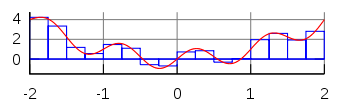
\includegraphics[width=7cm]{images/quadrature/int1}
b)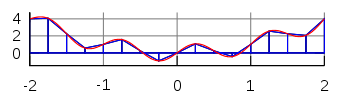
\includegraphics[width=7cm]{images/quadrature/int2}\\
The interval $[-2,2]$ is broken into 16 sub-intervals. The blue lines correspond to the 
approximation of the red curve by means of a) the midpoint rule,  b) the trapezoidal rule.
\end{center}

There are several algorithms for numerical integration (also commonly called ``{\color{olive}numerical quadrature}'', or
simply ``{\color{olive}quadrature}'') \index{general}{Quadrature}.
Interpolation with polynomials evaluated at equally spaced points in $[a,b]$
yields the Newton-Cotes formulas, of which the rectangle rule and the trapezoidal rule are examples. 
\index{general}{Newton-Cotes}

%-----------------------------
\subsubsection{in 1D - Gauss-Legendre quadrature  \label{sec:quad1Dglq}}

If we allow the intervals between interpolation points to vary, we find another group of quadrature formulas, such as 
the Gauss(ian) quadrature formulas. \index{general}{Gauss-Legendre Quadrature}
A Gaussian quadrature rule is typically more accurate than a Newton-Cotes rule, 
which requires the same number of function evaluations, if the integrand is smooth 
(i.e., if it is sufficiently differentiable).


An $n-$point Gaussian quadrature rule, named after Carl Friedrich Gauss, is a quadrature rule constructed
to yield an exact result for polynomials of degree $2n-1$ or less by a suitable choice of the points $x_i$
and weights $w_i$ for $i=1,\dots,n$.

The domain of integration for such a rule is conventionally taken as $[-1,1]$, so the rule is stated as
\begin{mdframed}[backgroundcolor=blue!5]
\[
\int_{-1}^{+1} f(x) dx = \sum_{i_q=1}^n w_{i_q} f(x_{i_q})
\]
\end{mdframed}
In this formula the $x_{i_q}$ coordinate is 
the $i$-th root of the {\color{olive} Legendre polynomial} $P_n(x)$\todo{what are these ?}. \index{general}{Legendre Polynomial}

It is important to note that a Gaussian quadrature will only produce good results if the function $f(x)$
is well approximated by a polynomial function within the range $[-1,1]$.
As a consequence, the method is not, for example, suitable for functions with singularities.

%\begin{center}
%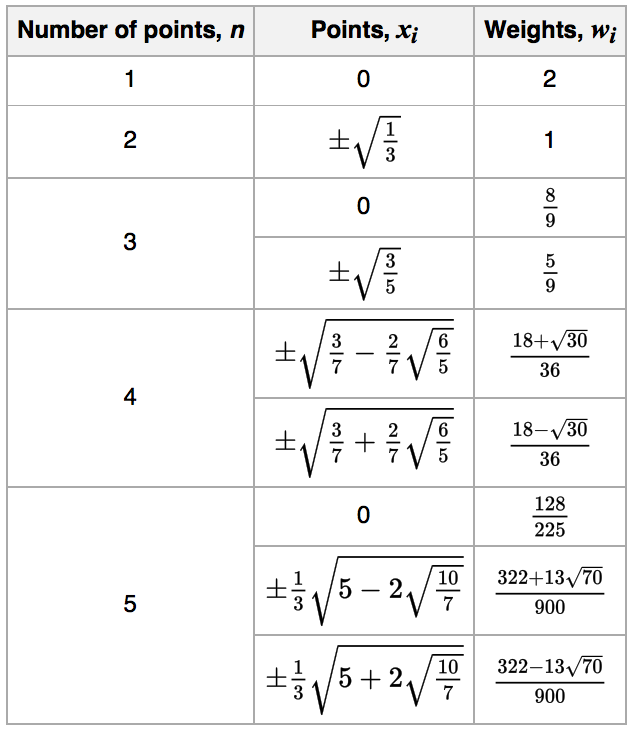
\includegraphics[width=5.cm]{images/quadrature/gq2}\\
%Gauss-Legendre points and their weights.
%\end{center}

\begin{center}
\begin{tabular}{lllrr}
\hline
n & $x_{iq}$ & $w_{iq}$ & $x_{iq}$ (approx) & $w_{iq}$ (approx) \\
\hline\hline
1 & 0 & 2 & 0 & 2 \\
\hline
2 & $\pm \sqrt{1/3}$ & 1  & $\pm$0.577 350 269 189 626 & 1 \\
\hline
3 & 0 & 8/9 & 0                                          & 0.888 888 888 888 888 \\
  & $\pm\sqrt{3/5}$  & 5/9  & $\pm$0.774 596 669 241 483 & 0.555 555 555 555 555 \\
\hline
4 & $\pm\sqrt{\frac{3}{7} - \frac{2}{7}\sqrt{6/5}}$  & $\frac{18+\sqrt{30}}{36}$ & $\pm$0.339 981 043 584 856 & 0.652 145 154 862 546 \\
  & $\pm\sqrt{\frac{3}{7} + \frac{2}{7}\sqrt{6/5}}$  & $\frac{18-\sqrt{30}}{36}$ & $\pm$0.861 136 311 594 953 & 0.347 854 845 137 454 \\
\hline
5 & 0 & 128/225                                    & 0                                                          & 0.568 888 888 888 889 \\
  & $\pm\frac{1}{3}\sqrt{5-2\sqrt{\frac{10}{7}}}$  & $\frac{322+13\sqrt{70}}{900}$ & $\pm$0.538 469 310 105 683 & 0.478 628 670 499 366 \\
  & $\pm\frac{1}{3}\sqrt{5+2\sqrt{\frac{10}{7}}}$  & $\frac{322-13\sqrt{70}}{900}$ & $\pm$0.906 179 845 938 664 & 0.236 926 885 056 189 \\
\hline
6 & ?& ?& $\pm$0.238 619 186 083 197 & 0.467 913 934 572 691\\
  &  &  & $\pm$0.661 209 386 466 265 & 0.360 761 573 048 139\\
  &  &  & $\pm$0.932 469 514 203 152 & 0.171 324 492 379 170\\
\hline
7 & & & $\pm$0.946 107 912 342 759 & 0.129 484 966 168 870\\
  & & & $\pm$0.741 531 185 599 394 & 0.279 705 391 489 277\\
  & & & $\pm$0.405 845 151 377 397 & 0.381 830 050 505 119\\
  & & & 0.000 000 000 000 000 & 0.417 959 183 673 469\\
\hline
8 & & & $\pm$0.960 289 856 497 536 & 0.101 228 536 290 376\\
  & & & $\pm$0.796 666 477 413 627 & 0.222 381 034 453 374\\
  & & & $\pm$0.525 532 409 916 329 & 0.313 706 645 877 887\\
  & & & $\pm$0.183 434 642 495 650 & 0.362 683 783 378 362\\
\hline
9 & & & $\pm$0.968 160 239 507 626 & 0.081 274 388 361 574\\
  & & & $\pm$0.836 031 107 326 636 & 0.180 648 160 694 857\\
  & & & $\pm$0.613 371 432 700 590 & 0.260 610 696 402 935\\
  & & & $\pm$0.324 253 423 403 809 & 0.312 347 077 040 003\\
  & & & 0.000 000 000 000 000 & 0.330 239 355 001 260\\
\hline
10 &&& $\pm$0.973 906 528 517 172 & 0.066 671 344 308 688\\
   &&& $\pm$0.865 063 366 688 985 & 0.149 451 349 150 581\\
   &&& $\pm$0.679 409 568 299 024 & 0.219 086 362 515 982\\
   &&& $\pm$0.433 395 394 129 247 & 0.269 266 719 309 996\\
   &&& $\pm$0.148 874 338 981 631 & 0.295 524 224 714 753\\
\hline
\end{tabular}\\
{\captionfont Abscissae and weights for Gauss quadratures up to $n=10$. See \cite[p89]{li06}}
\end{center}

As shown in the above table, it can be shown that the weight values must fulfil the following condition:
\begin{equation}
\sum_{i_q} w_{i_q}=2 \label{gq23}
\end{equation}
This simply comes from the requirement that when $f(x)=1$ then $\int_{-1}^{+1}f(x)dx=2=\sum w_{iq}$.
It is also worth noting that all quadrature point coordinates are symmetrical around the origin.

Since most quadrature formula are only valid on a specific interval, we now must address the problem 
of their use outside of such intervals. The solution turns out to be quite simple: one 
must carry out a change of variables from the interval $[a,b]$ to $[-1,1]$.
We then consider the reduced coordinate $r\in[-1,1]$ such that 
\begin{equation}
r=\frac{2}{b-a}(x-a)-1 
\end{equation}
This relationship can be reversed such that when $r$ is known, its equivalent coordinate 
$x\in[a,b]$ can be computed:
\begin{equation}
x=\frac{b-a}{2}(1+r)+a
\end{equation}
From this it follows that
\begin{equation}
dx=\frac{b-a}{2}dr
\end{equation}
and then 
\begin{mdframed}[backgroundcolor=blue!5]
\begin{equation}
\int_a^b f(x) dx  = \frac{b-a}{2} \int_{-1}^{+1} f(r) dr \simeq 
\frac{b-a}{2} \sum_{i_q=1}^{n_q} w_{i_q} f(r_{i_q})
\end{equation}
\end{mdframed}

%--------------------
\subsubsection{A probably naive way of finding the quadrature points coordinates and weights}

We start from the assumption that the quadrature must be exact for polynomials $f(r)$, that it is 
written
\[
I= \int_{-1}^{+1} f(r) dr = \sum_{i_q=1}^{n_q} w_{iq} f(r_{i_q}) 
\]
and that $n_q>0$, $w_{i_q}\neq 0$ and $r_{i_q}\in [-1,1]$.

Let us start with zero-th order polynomials, i.e. $f(r)=C$. Then $I=2C$ and we must then 
have 
\[
2C = \sum_{i_q=1}^{n_q} w_{iq} f(r_{i_q})  =  \sum_{i_q=1}^{n_q} w_{iq} C   
\]
which imposes 
\begin{equation}
\boxed{
\sum_{i_q=1}^{n_q} w_{iq} = 2 \qquad \forall n_q>0
}
\label{eq:glqone}
\end{equation}
As long as the sum of the weights is equal to 2, any $n_q$-point based quadrature can 
integrate exactly a zero-th order polynomial. 

Let us move on with first-order polynomials. Since we have covered the constant term hereabove, we
set $f(r)=ar$ where $a\neq 0$. We have $I=0$ so
\begin{equation}
0 = \sum_{i_q=1}^{n_q} w_{iq} f(r_{i_q})  = a \sum_{i_q=1}^{n_q} w_{iq} r_{i_q}
\qquad
\Rightarrow
\qquad
\boxed{
\sum_{i_q=1}^{n_q} w_{iq} r_{i_q} = 0\qquad \forall n_q>0
}
 \label{eq:glqtwo}
\end{equation}
In order to integrate exactly first-order polynomials an $n_q$-point based quadrature must 
fulfil Eqs.\eqref{eq:glqone} and \eqref{eq:glqtwo}.
\begin{itemize}
\item
If $n_q=1$, then we automatically have $w_1=2$ and $w_1 r_1 =0 $, i.e. $r_1=0$.
\item
If $n_q=2$, then $w_1+w_2=2$ and $w_1r_1+w_2r_2 = 0$. There are many solutions $w_1,w_2,r_1,r_2$ which 
can fulfil these two equations, so this is not enough to determine a unique set of coordinates and weights.
\end{itemize}

Let us now turn to second-order polynomials: as before, I choose $f(r)=a r^2$. We have 
$I=2a/3$ and 
\begin{equation}
\frac{2a}{3} = \sum_{i_q=1}^{n_q} w_{iq} f(r_{i_q})  = a \sum_{i_q=1}^{n_q} w_{iq} r_{i_q}^2 
\qquad
\boxed{
\sum_{i_q=1}^{n_q} w_{iq} r^2_{i_q} = \frac{2}{3}\qquad \forall n_q>0
}
\label{eq:glqthree}
\end{equation}
\begin{itemize}
\item
If $n_q=1$, we know that $w_1=2$ and $r_1=0$. 
This means that 1-point quadrature cannot exactly integrate polynomials higher than 1.
\item
If $n_q=2$, then $w_1+w_2=2$, $w_1r_1+w_2r_2 =0$ and now $w_1r_1^2+w_2r_2^2 =2/3$. We have three equations but still four unknowns. 
At this stage, we can do a simple additional assumption: common sense would have us realise that there is no 
reason why the (in this case) 2 quadrature point coordinates should be both negative or both positive. In light 
thereof we require that quadrature point coordinates are symmetric with respect with the origin $r=0$, i.e. $r_1=-r_2$ in this case.
This yields to write:  $w_1r_1+w_2r_2 = w_1r_1+w_2(-r_1)=r_1(w_1-w_2)=0$. If $r_1=0$ then $r_2=0$ too and we do not 
have a 2-point quadrature. It must then follows that $w_1=w_2$. And finally 
$w_1r_1^2+w_2r_2^2 = w_1 r_1^2 + w_1 (-r_1)^2=2/3$, i.e. $r_1=-1/\sqrt{3}$ and $r_2=1/\sqrt{3}$ since $r_1<r_2$.
\end{itemize}

If we now turn to third-order polynomials, i.e. $f(r)=ar^3$, then $I=0$ again. We then must have
\begin{equation}
\boxed{
\sum_{i_q=1}^{n_q} w_{iq} r^3_{i_q} =  0  \qquad \forall n_q>0
}
\end{equation}
We see that the coordinates and weights obtained for a 2-point quadrature verify this equation, i.e. 
a 2-point quadrature can also exactly integrate a 3rd-order polynomial.
However, it is equally easy to verify that the 2-point quadrature cannot exactly integrate a 4th-order polynomial
since 
\[
I= \int_{-1}^{+1} r^4 dr = \frac{2}{5} \neq  \sum_{i_q=1}^{2} w_{iq} r_{i_q}^4
\]
A three-point quadrature will then be needed for those. Because of the symmetry, we know that the middle
point will be at $r=0$.

\begin{remark} 
This approach unfortunately does not shed any light on why the method is called Gauss-Legendre quadrature
nor why the quadrature points are the zeros of the Legendre polynomials...
\end{remark}


%--------------------
\subsubsection{in 1D - examples}

\paragraph{example 1}

Since we know how to carry out any required change of variables, we choose for simplicity 
$a=-1$, $b=+1$.
Let us take for example $f(r)=\pi$. Then we can compute the integral of this function 
over the interval $[a,b]$ exactly:
\[
I=\int_{-1}^{+1} f(r) dr = \pi \int_{-1}^{+1}dr  = 2 \pi
\]
We can now use a Gauss-Legendre formula to compute this same integral:
\[
I_{gq}=\int_{-1}^{+1} f(r) dr
= \sum_{i_q=1}^{n_q} w_{i_q} f(r_{i_q}) 
= \sum_{i_q=1}^{n_q} w_{i_q} \pi
= \pi \underbrace{\sum_{i_q=1}^{n_q} w_{i_q} }_{=2}
= 2 \pi
\]
where we have used the property of the weight values of Eq.(\ref{gq23}).
Since the actual number of points was never specified, this result is valid for all 
quadrature rules.


\paragraph{example 2}

Let us now take $f(r)=m r+ p$ and repeat the same exercise:
\[
I=\int_{-1}^{+1} f(r) dr = \int_{-1}^{+1} (mr+p) dr  =  [\frac{1}{2} m r^2 + p r ]_{-1}^{+1} =2p
\]
\[
I_{gq}=\int_{-1}^{+1} f(r) dr
\!= \sum_{i_q=1}^{n_q} w_{i_q} f(r_{i_q}) 
\!= \sum_{i_q=1}^{n_q} w_{i_q} (m r_{i_q} + p)  
\!= m \underbrace{\sum_{i_q=1}^{n_q} w_{i_q} r_{i_q}}_{=0}  + p \underbrace{\sum_{i_q=1}^{n_q} w_{i_q}}_{=2}  = 2p
\]
since the quadrature points are symmetric w.r.t. to zero on the $r$-axis.
Once again the quadrature is able to compute the exact value of this integral: this makes sense since 
an $n$-point rule exactly integrates a $2n-1$ order polynomial such that a 1 point quadrature exactly 
integrates a first order polynomial like the one above.



\paragraph{example 3}

Let us now take $f(r)=r^2$. We have 
\[
I=\int_{-1}^{+1} f(r) dr = \int_{-1}^{+1} r^2 dr  =  \left[\frac{1}{3}r^3 \right]_{-1}^{+1} =  \frac{2}{3} 
\]
and 
\[
I_{gq}=\int_{-1}^{+1} f(r) dr 
\!= \sum_{i_q=1}^{n_q} w_{i_q} f(r_{i_q}) 
\!= \sum_{i_q=1}^{n_q} w_{i_q} r_{i_q}^2 
\]

\begin{itemize}
\item $n_q=1$: $r_{iq}^{(1)}=0$, $w_{i_q}=2$. $I_{gq}=0$
\item $n_q=2$: $r_{q}^{(1)}=-1/\sqrt{3}$, $r_{q}^{(2)}=1/\sqrt{3}$, $w_{q}^{(1)}=w_{q}^{(2)}=1$. $I_{gq}=\frac{2}{3}$
\item It also works $\forall n_q>2$ !
\end{itemize}

%-----------------------------
\subsubsection{in 2D/3D - theory}

Let us now turn to a two-dimensional integral of the form
\[
I=\int_{-1}^{+1} \int_{-1}^{+1} f(r,s) dr ds
\]
where $f(r,s)$ is again assumed to be continuous over the domain. 
The equivalent Gaussian quadrature writes:
\[
I_{gq}
\simeq \sum_{i_q=1}^{n_q}\sum_{j_q}^{n_q} f(r_{i_q},s_{j_q}) w_{i_q} w_{j_q}
\]
Finally we have 
\begin{mdframed}[backgroundcolor=blue!5]
\begin{equation}
I=\int_{a}^{+b}\int_{c}^{+d} f(r,s) dr ds
\simeq \frac{b-a}{2} \frac{d-c}{2} 
\sum_{i_q=1}^{n_q}\sum_{j_q}^{n_q} f(r_{i_q},s_{j_q}) w_{i_q} w_{j_q}
\end{equation}
\end{mdframed}

%----------------------------------------
\subsubsection{Quadrature on triangles}
\begin{flushright} {\tiny {\color{gray} quadrature\_triangles.tex}} \end{flushright}
%~~~~~~~~~~~~~~~~~~~~~~~~~~~~~~~~~~~~~~~~~~~~~~~~~~~~~~~~~~~~~~~~~~~~~~~~~~~~~~~~~~~~~~~~~~~~~~~~~~

Quadrature rules for triangles can be found in \textcite{duna85} (1985).
The following ones are identical to those in the {\sl ip\_triangle.m} 
file of the MILAMIN code \cite{daks08}. See also \textcite{leth76} (1976)
on the topic of computation of double integrals over a triangle.

{\small
\[
\begin{array}{c|ccc|ccc}
\hline
&r_q & s_q & w_q &r_q & s_q & w_q \\ 
&\text{exact} & \text{exact} & \text{exact} & \text{approx.}& \text{approx.}& \text{approx.}\\
\hline\hline
iq=1& 1/3 & 1/3 & 1/2\\
\hline
iq=1 & 1/6 & 1/6 & 1/6 \\
iq=2 & 2/3 & 1/6 & 1/6 \\
iq=3 & 1/6 & 2/3 & 1/6 \\
\hline
iq=1&1/3 & 1/3 & -27/96\\
iq=2&0.6 & 0.2 &  25/96\\
iq=3&0.2 & 0.6 &  25/96\\
iq=4&0.2 & 0.2 &  25/96\\
\hline
iq=1& 1-2g_1 & g_1 & w_1/2  &  0.108103018168070 & 0.44594849091596  &   \\
iq=2& g_1 & 1-2g_1 & w_1/2  &  0.445948490915965 & 0.108103018168070 &   \\
iq=3& g_1 & g_1    & w_1/2  &  0.445948490915965 & 0.445948490915965 &   \\
iq=4& 1-2g_2 & g_2 & w_2/2  &  0.816847572980459 & 0.091576213509771 &   \\
iq=5& g_2 & 1-2g_2 & w_2/2  &  0.091576213509771 & 0.816847572980459 &   \\
iq=6& g_2 & g_2    & w_2/2  &  0.091576213509771 & 0.091576213509771 &   \\
\hline
iq=1&&&&0.091576213509771 &  0.091576213509771    &    0.109951743655322/2.0 \\ 
iq=2&&&&0.816847572980459 &  0.091576213509771    &    0.109951743655322/2.0 \\
iq=3&&&&0.091576213509771 &  0.816847572980459    &    0.109951743655322/2.0 \\
iq=4&&&&0.445948490915965 &  0.445948490915965    &    0.223381589678011/2.0 \\
iq=5&&&&0.108103018168070 &  0.445948490915965    &    0.223381589678011/2.0 \\
iq=6&&&&0.445948490915965 &  0.108103018168070    &    0.223381589678011/2.0 \\
\hline
iq=1 &&&&0.1012865073235 &  0.1012865073235  &     0.0629695902724 \\
iq=2 &&&&0.7974269853531 &  0.1012865073235  &     0.0629695902724 \\
iq=3 &&&&0.1012865073235 &  0.7974269853531  &     0.0629695902724 \\
iq=4 &&&&0.4701420641051 &  0.0597158717898  &     0.0661970763942 \\
iq=5 &&&&0.4701420641051 &  0.4701420641051  &     0.0661970763942 \\
iq=6 &&&&0.0597158717898 &  0.4701420641051  &     0.0661970763942 \\
iq=7 &&&&0.3333333333333 &  0.3333333333333  &     0.1125000000000 \\
\hline
iq=1&&&& 5.01426509658179e-01&  2.49286745170910e-01 &   5.83931378631895e-02 \\ 
iq=2&&&& 2.49286745170910e-01&  5.01426509658179e-01 &   5.83931378631895e-02 \\ 
iq=3&&&& 2.49286745170910e-01&  2.49286745170910e-01 &   5.83931378631895e-02 \\ 
iq=4&&&& 8.73821971016996e-01&  6.30890144915020e-02 &   2.54224531851035e-02 \\ 
iq=5&&&& 6.30890144915020e-02&  8.73821971016996e-01 &   2.54224531851035e-02 \\ 
iq=6&&&& 6.30890144915020e-02&  6.30890144915020e-02 &   2.54224531851035e-02 \\ 
iq=7&&&& 5.31450498448170e-02&  3.10352451033784e-01 &   4.14255378091870e-02 \\ 
iq=8&&&& 6.36502499121399e-01&  5.31450498448170e-02 &   4.14255378091870e-02 \\ 
iq=9&&&& 3.10352451033784e-01&  6.36502499121399e-01 &   4.14255378091870e-02 \\ 
iq=10&&&& 5.31450498448170e-02&  6.36502499121399e-01 &   4.14255378091870e-02 \\ 
iq=11&&&& 6.36502499121399e-01&  3.10352451033784e-01 &   4.14255378091870e-02 \\ 
iq=12&&&& 3.10352451033784e-01&  5.31450498448170e-02 &   4.14255378091870e-02 \\ 
\hline
\end{array}
\]
}
where
\[ 
g_1 = \left(8-\sqrt{10} + \sqrt{38-44\sqrt{2/5}}\right)/18
\qquad
g_2 = \left(8-\sqrt{10} - \sqrt{38-44\sqrt{2/5}}\right)/18
\]
\[
w_1 = \left(620+\sqrt{213125-53320\sqrt{10}}\right)/3720
\qquad
w_2 = \left(620-\sqrt{213125-53320\sqrt{10}}\right)/3720
\]

Note that when 4 points are used one of the weights is negative?










%----------------------------------------
\subsubsection{A mathematical recreation: computing the volume of a tetrahedron}

Let us find the volume of tetrahedron bounded by the planes passing through the points 
A(1,0,0), B(0,1,0), C(0,0,1) and the coordinate planes Oxy, Oxz and Oyz.

\begin{flushright} {\tiny {\color{gray} (tikz\_tetrahedron.tex)}} \end{flushright}
%~~~~~~~~~~~~~~~~~~~~~~~~~~~~~~~~~~~~~~~~~~~~~~~~~~~~~~~~~~~~~~~~~~~~~~~~~~~~~~~~~~~~~~~~~~~~~~~~~~
\begin{center}
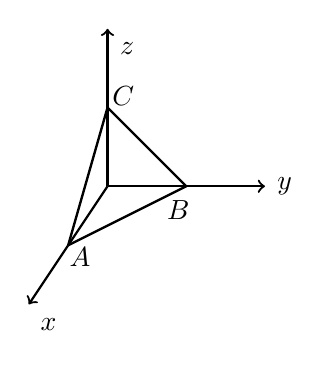
\begin{tikzpicture}
%\draw[step=0.5cm,gray,very thin] (0,0) grid (4,4); %background grid

\draw [thick,->] (1.5,2) -- (3.5,2);
\draw [thick,->] (1.5,2) -- (1.5,4);
\draw [thick,->] (1.5,2) -- (0.5,0.5);

\node[] at (0.75,0.25) {$x$};
\node[] at (3.75,2) {$y$};
\node[] at (1.75,3.75) {$z$};

\draw[line width=0.3mm] (1,1.25) -- (2.5,2) ;   
\node[] at (2.4,1.7) {$B$};

\draw[line width=0.3mm] (2.5,2) -- (1.5,3) ;   
\node[] at (1.7,3.15) {$C$};

\draw[line width=0.3mm] (1.5,3) -- (1,1.25) ;   
\node[] at (1.15,1.1) {$A$};

\end{tikzpicture}
\end{center}


The equation of the plane is $x+y+z=1$, or $z=1-x-y$.Hence, the limits of integration over 
the variable $z$ range in the interval from
$z=0$ to $z=1-x-y$. Now we can calculate the volume of the tetrahedron:
\begin{eqnarray}
V 
&=& \iiint dx \; dy \; dz \nn\\
&=& \int_0^1 dx \int_0^{1-x} dy \int_{0}^{1-x-y} dz \nn\\
&=& \int_0^1 dx \int_0^{1-x} dy (1-x-y) \nn\\
&=& \int_0^1 dx \left[y-xy-\frac12 y^2 \right]_0^{1-x} \nn\\
&=& \int_0^1 dx \left((1-x)-x(1-x)-\frac12 (1-x)^2 \right) \nn\\
&=& \int_0^1 dx \left(\frac12 -x + \frac12 x^2   \right) \nn\\
&=& \left[ \frac12 x  -\frac12 x^2 + \frac16 x^3   \right]_0^1 \nn\\
&=& \frac16
\end{eqnarray}
We will use this result in the following section.

%----------------------------------------
\subsubsection{Quadrature on tetrahedra}

\begin{remark}
In what follows the coefficients in the tables are not the reduced coordinates
of the quadratue points but the coefficients corresponding to the 4 nodes.
\end{remark}

Quadrature rules on tetrahedra take the form:
\[
\int\int\int_{el} f(x,y,z) dxdydz = V_{el} \sum_{iq=1}^{nqel} 
w_{iq} f(\xi^{iq}_1,\xi^{iq}_2,\xi^{iq}_3,\xi^{iq}_4) 
\]
or, that is to say:
\[
\int\int\int_{el} f(x,y,z) dxdydz = \sum_{iq=1}^{nqel} 
(w_{iq}V_{el}) f(\xi^{iq}_1,\xi^{iq}_2,\xi^{iq}_3,\xi^{iq}_4) 
\]
with in our case $V_{el}=1/6$.

In the literature it can be found that a one point quadrature is characterised by 
\[
w_{iq}=1 \quad\quad\quad \xi^{iq}_1=\xi^{iq}_2=\xi^{iq}_3=\xi^{iq}_4=0.25
\]
i.e, the coordinates of the single point are given by:
\[
x_{iq}=\sum_{i=1}^4 \xi_i^{iq} x_i = \frac{1}{4} (x_1+x_2+x_3+x_4)
\]
Same for $y$ and $z$ coordinates. 

A four-point quadrature rule is characterised by $w_{iq}=V_{el}*0.25=1/24\simeq 04166666666666667$ and 

\begin{tabular}{lcccc}
\hline
 & $\xi_1$ & $\xi_2$ & $\xi_3$ & $\xi_4$ \\
\hline\hline
iq=1 & 0.585410196624969 & 0.138196601125011 & 0.138196601125011 & 0.138196601125011 \\
iq=2 & 0.138196601125011 & 0.585410196624969 & 0.138196601125011 & 0.138196601125011 \\
iq=3 & 0.138196601125011 & 0.138196601125011 & 0.585410196624969 & 0.138196601125011 \\
iq=4 & 0.138196601125011 & 0.138196601125011 & 0.138196601125011 & 0.585410196624969 \\
\hline
\end{tabular}

We then have:
\[
r_{iq}=\sum_{i=1}^4 \xi_i^{iq} x_i 
= (\xi_1^{iq},\xi_2^{iq},\xi_3^{iq},\xi_4^{iq})\cdot(r_1,r_2,r_3,r_4) 
= (\xi_1^{iq},\xi_2^{iq},\xi_3^{iq},\xi_4^{iq})\cdot(0,1,0,0) 
= \xi_2^{iq}
\]
\[
s_{iq}=\sum_{i=1}^4 \xi_i^{iq} y_i 
= (\xi_1^{iq},\xi_2^{iq},\xi_3^{iq},\xi_4^{iq})\cdot(s_1,s_2,s_3,s_4) 
= (\xi_1^{iq},\xi_2^{iq},\xi_3^{iq},\xi_4^{iq})\cdot(0,0,1,0) 
= \xi_3^{iq}
\]
\[
t_{iq}=\sum_{i=1}^4 \xi_i^{iq} z_i 
= (\xi_1^{iq},\xi_2^{iq},\xi_3^{iq},\xi_4^{iq})\cdot(t_1,t_2,t_3,t_4) 
= (\xi_1^{iq},\xi_2^{iq},\xi_3^{iq},\xi_4^{iq})\cdot(0,0,0,1) 
= \xi_4^{iq}
\]
Finally:

\begin{tabular}{ccccc}
\hline
     & $r_q$ & $s_q$ & $t_q$  & $w_q$ \\
\hline
\hline
iq=1 & 0.138196601125011 & 0.138196601125011 & 0.138196601125011 & 0.04166666666666667\\
iq=2 & 0.585410196624969 & 0.138196601125011 & 0.138196601125011 & 0.04166666666666667\\
iq=3 & 0.138196601125011 & 0.585410196624969 & 0.138196601125011 & 0.04166666666666667\\
iq=4 & 0.138196601125011 & 0.138196601125011 & 0.585410196624969 & 0.04166666666666667\\
\hline
\end{tabular}


%------------------------------------------
\subsubsection{The Gauss-Lobatto approach \label{sec:loba}}

All what we have seen above falls under the Gauss-Legendre quadrature method. There is however another 
somewhat common quadrature method: the Gauss-Lobatto  quadrature. \index{general}{Gauss-Lobatto}.
It is similar to Gaussian quadrature with the following  important differences:
1) There are integration points in the interval but they also always include the end points of the integration interval;
2) It is accurate for polynomials up to degree $2n-3$, where $n$ is the number of integration points.

In 1D, it reads:
\[
\int_{-1}^{+1} f(x) dx = \frac{2}{n(n-1)} [f(-1)+f(1)] + \sum_{i=2}^{n-1} w_i f(x_i) 
\]
The locations and weights of the integration points are as follows:

\begin{center}
\begin{tabular}{lllll}
\hline
n & $x_{iq}$ & $w_{iq}$ & $x_{iq}$ (approx) & $w_{iq}$ (approx) \\
\hline\hline
3 & 0 & 4/3 & & \\
  & $\pm 1$ & 1/3 & &  \\
\hline
4 & $\pm\sqrt{\frac{1}{5}}$ & 5/6 & & \\
  & $\pm 1$ & 1/6 & & \\
\hline
5 & 0 & 32/45 & & \\
  & $\pm\sqrt{\frac{3}{7}}$ & 49/90 & & \\
  & $\pm 1$ & 1/10 & & \\
\hline
6 & $\pm\sqrt{\frac{1}{3} -\frac{2\sqrt{7}}{21}}$ & $\frac{14+\sqrt{7}}{30}$ & & \\
  & $\pm\sqrt{\frac{1}{3} +\frac{2\sqrt{7}}{21}}$ & $\frac{14-\sqrt{7}}{30}$ & & \\
  & $\pm 1$ & 1/15 \\
\hline
\end{tabular}
\end{center}

 
%-------------------------------------------------------------------------
\subsubsection{Computing the 'real' coordinates of the quadrature points and other considerations}

The quadrature point coordinates are always given in (what I call) reduced coordinates, i.e. between 
-1 and 1.
However, one sometimes need their equivalent in the $x,y$ Cartesian space. 
This is trivial once one remembers that within an element, a field $f$ is reprensented 
as follow:
\[
f(r,s) = \sum_{i=1}^{m} \bN_{i}(r,s) f_i
\]
where $m$ is the number of nodes, $r$ and $s$ are the reduced coordinates 
and $\bN_i$ are the basis functions. 
The value of $f$ at a quadrature point $(r_q,s_q)$ is then simply
\[
f(r_q,s_q) = \sum_{i=1}^{m} \bN_{i}(r_q,s_q) f_i
\]
If we now take $f=x$, then
\[
x_q =x(r_q,s_q) = \sum_{i=1}^{m} \bN_{i}(r_q,s_q) x_i
\]
and
\[
y_q =y(r_q,s_q) = \sum_{i=1}^{m} \bN_{i}(r_q,s_q) y_i
\]
where $x_i$ and $y_i$ are the Cartesian coordinates of the nodes.
This is then easily extended to three dimensions:
\[
x_q =x(r_q,s_q,t_q) = \sum_{i=1}^{m} \bN_{i}(r_q,s_q,t_q) x_i
\]
\[
y_q =x(r_q,s_q,t_q) = \sum_{i=1}^{m} \bN_{i}(r_q,s_q,t_q) y_i
\]
\[
z_q =z(r_q,s_q,t_q) = \sum_{i=1}^{m} \bN_{i}(r_q,s_q,t_q) z_i
\]
or, 
\[
\vec{r}_q =\vec{r}(r_q,s_q,t_q) = \sum_{i=1}^{m} \bN_{i}(r_q,s_q,t_q) \vec{r}_i
\]
This also applies to other fields such as velocity, temperature, or even strain rate components 
(as long as the strain rate values have previously been computed on the nodes): 
\[
\vec{\upnu}_q =\vec{\upnu}(r_q,s_q) = \sum_{i=1}^{m} \bN_{i}(r_q,s_q) \vec{\upnu}_i
\]
\[
T_q =T(r_q,s_q) = \sum_{i=1}^{m} \bN_{i}(r_q,s_q) T_i
\]
\[
\dot{\varepsilon}_{xy,q} 
= \dot{\varepsilon}_{xy} (r_q,s_q) = \sum_{i=1}^{m} \bN_{i}(r_q,s_q)  \dot{\varepsilon}_{xy,i}
\]













